\documentclass[11pt,a4paper]{article}
\usepackage[margin=2.4cm]{geometry}
\usepackage{amsmath,amssymb,bm}
\usepackage{graphicx}
\usepackage{booktabs}
\usepackage[colorlinks=true,linkcolor=blue,citecolor=blue]{hyperref}
\usepackage{xcolor}

\newcommand{\dt}{\partial_t}
\newcommand{\dx}{\partial_x}
\newcommand{\dy}{\partial_y}
\newcommand{\dn}{\partial_n}
\newcommand{\ds}{\partial_s}
\newcommand{\code}[1]{\texttt{\small #1}}

\title{Every equation solved by \code{funwave\_2d\_sw/run\_meander.py}\\
\large Nonlinear depth-averaged shallow water on a meandering channel\\
with an erodible bed and erodible banks}
\author{\code{rossby\_palooza/numerical/funwave\_2d\_sw}}
\date{2026-07-22}

\begin{document}
\maketitle

\begin{abstract}
\noindent
This note writes down, without omission, the system that the driver
\code{run\_meander.py} sets up and that FUNWAVE-TVD integrates: the interior mass and
momentum equations, every closure, how a sinuous channel is prescribed on a Cartesian
grid, the boundary conditions (hydrodynamic and sedimentary), the initial condition, the
bed-evolution equation, and the bank treatment. Numbers quoted are the values actually
in \code{CONFIG}; the figures are generated from the driver itself by
\code{make\_figs.py}, so this document cannot drift from the code. What the model does
\emph{not} contain is stated in \S\ref{sec:notcontain}, because that bounds every result.
\end{abstract}

\tableofcontents

% =====================================================================
\section{Scope and sign conventions}

Independent variables are the down-valley coordinate $x$, the cross-valley coordinate
$y$, and time $t$. All fields are \textbf{depth-averaged}: there is no vertical
coordinate and no vertical structure. Dependent variables:

\begin{center}
\begin{tabular}{lll}
\toprule
symbol & meaning & sign \\
\midrule
$\eta(x,y,t)$ & free-surface elevation above the still-water datum & up $+$ \\
$h(x,y,t)$ & still-water depth & down $+$ \\
$H=\eta+h$ & total water depth & $\ge 0$ \\
$(u,v)$ & depth-averaged velocity & \\
$(P,Q)=(Hu,Hv)$ & volume flux per unit width & \\
$\bar c(x,y,t)$ & depth-averaged volumetric sediment concentration & \\
$z_b=-h$ & bed elevation & up $+$ \\
\bottomrule
\end{tabular}
\end{center}

\noindent
\textbf{A trap worth stating once.} FUNWAVE's internal bed-change variable \code{Zb} is
\emph{positive for erosion} and enters as \code{Depth = Depth\_ini + Zb*Morph\_factor}.
Erosion therefore \emph{increases} \code{Depth} and \emph{decreases} $z_b$.

% =====================================================================
\section{Interior equations}

\subsection{Mass}
\begin{equation}
  \dt\eta + \dx(Hu) + \dy(Hv) \;=\; -\,\dt h .
  \label{eq:mass}
\end{equation}
The right-hand side is the coupling to the moving bed: a rising bed displaces water. Under
the morphodynamic scale separation of \S\ref{sec:timescales} it is dropped from the
hydrodynamic step and reinstated only when the bed is updated.

\subsection{Momentum}
In conservative, well-balanced form --- which is what FUNWAVE integrates once
\code{DISPERSION = F} sets $\Gamma_1=\Gamma_2=0$ (\code{src/init.F:647-652}):
\begin{align}
  \dt P + \dx\!\left[\frac{P^2}{H} + \tfrac12 g\!\left(\eta^2+2\eta h\right)\right]
        + \dy\!\left[\frac{PQ}{H}\right]
  &= g\eta\,\dx h \;-\; C_d\,u\sqrt{u^2+v^2} \;+\; \nabla\!\cdot\!\left(\nu_t H\nabla u\right),
  \label{eq:momx}\\[2pt]
  \dt Q + \dx\!\left[\frac{PQ}{H}\right]
        + \dy\!\left[\frac{Q^2}{H} + \tfrac12 g\!\left(\eta^2+2\eta h\right)\right]
  &= g\eta\,\dy h \;-\; C_d\,v\sqrt{u^2+v^2} \;+\; \nabla\!\cdot\!\left(\nu_t H\nabla v\right).
  \label{eq:momy}
\end{align}

Splitting the hydrostatic pressure as $\tfrac12 g(\eta^2+2\eta h)$ with the source
$g\eta\,\nabla h$ is what makes the scheme \emph{well-balanced}: lake-at-rest
($\eta\equiv0$, $\bm u\equiv 0$) is preserved exactly over an arbitrary bed. This matters
here because the bed is strongly non-flat by construction.

\subsection{Closures}
\begin{align}
  \text{bed friction (\code{src/sources.F:242})}\qquad
  &\bm\tau_b/\rho = C_d\,\bm u\,|\bm u| , \label{eq:fric}\\
  \text{lateral mixing (\code{src/sources.F:367-385})}\qquad
  &\nu_t = C_{\rm smg}\,\Delta x\,\Delta y\,
     \sqrt{u_x^2+v_y^2+\tfrac12(u_y+v_x)^2} \;+\; \nu_{\rm bkg}. \label{eq:smag}
\end{align}
with $C_{\rm smg}=0.25$ (\code{src/mod\_global.F:301}) and $\nu_{\rm bkg}=0$.

\paragraph{$C_d$ is not free.} FUNWAVE's sediment module computes its own bed shear from a
log law (\S\ref{sec:sed}) that is \emph{independent} of the \code{Cd} in \code{input.txt}.
Consistency requires setting
\begin{equation}
  C_d \;=\; \frac{\kappa^2}{\left[\ln(30H/k_s)-1\right]^2}
  \;=\; 0.00154 \qquad (H=3\;\mathrm{m},\ k_s=2.5D_{50},\ D_{50}=0.5\;\mathrm{mm}).
  \label{eq:cd}
\end{equation}
Leaving the shipped example's $0.002$ makes flow and transport see a bed that differs by
$30\%$.

\paragraph{Relation to the linear $(s,n)$ model.} Linearising \eqref{eq:fric} about a base
state $(\bar U,0)$ with $H=\bar H+\eta'$ gives
\begin{equation}
  \frac{C_d\,\bm u|\bm u|}{H}\Big|_{x} \simeq
  \underbrace{\frac{C_d\bar U^2}{\bar H}}_{\text{base}}
  + \underbrace{\frac{2C_d\bar U}{\bar H}}_{r_s}u'
  - \underbrace{\frac{C_d\bar U^2}{\bar H^2}}_{r_\eta}\eta' ,
  \qquad
  \frac{C_d\,\bm u|\bm u|}{H}\Big|_{y} \simeq
  \underbrace{\frac{C_d\bar U}{\bar H}}_{r_n}v' .
\end{equation}
So the anisotropic drag $r_s=2C_f\bar U/\bar H$, $r_n=C_f\bar U/\bar H$ and the
superelevation-drag $r_\eta=C_f\bar U^2/\bar H^2$ of the $(s,n)$ linear model are
\emph{exactly} the first-order expansion of the single term \eqref{eq:fric}. The two
models agree on friction to first order; FUNWAVE additionally carries all higher orders.

% =====================================================================
\section{Geometry: prescribing a sinuous channel on a Cartesian grid}
\label{sec:geom}

FUNWAVE has no curvilinear option, so the meander lives entirely in the bathymetry
$h(x,y)$. Three steps.

\subsection{Centreline, with a straight lead-in}
\begin{equation}
  y_c(x) \;=\; A\,T(x)\,\cos(kx), \qquad k=\frac{2\pi}{\lambda},
  \label{eq:centreline}
\end{equation}
where $T$ is a raised-cosine amplitude taper that is identically zero over a straight
lead-in of length $\ell_s$ and reaches one at the edge of the buffer $\ell_b$:
\begin{equation}
  T(x)=\tfrac12\left[1-\cos\!\left(\pi\,\Pi\!\left(\frac{d(x)-\ell_s}{\ell_b-\ell_s}\right)\right)\right],
  \qquad d(x)=\min\big(x,\;L-x\big),
  \label{eq:taper}
\end{equation}
$\Pi$ denoting clipping to $[0,1]$. Both position and slope are continuous at the joins,
and $y_c(0)=y_c(L)=0$: \textbf{both ends of the domain sit on the valley axis, in a dead
straight channel}. The reason is boundary conditions, \S\ref{sec:bc}: the tide sponge is
30 cells wide and the state it imposes ($u=U$, $v=0$, $\eta$ constant) is exactly correct
only in a uniform straight reach.

\paragraph{Curvature.} Because of the taper the analytic curvature of $A\cos kx$ no longer
applies, so the signed curvature is taken by finite difference on the sampled curve,
\begin{equation}
  \kappa \;=\; \frac{x'y''-y'x''}{\left(x'^2+y'^2\right)^{3/2}} .
  \label{eq:kappa}
\end{equation}
In the interior $|\kappa|_{\max}\to C_0\equiv Ak^2$; inside the sponge it is $2$--$8\%$ of
$C_0$.

\subsection{Channel coordinates by nearest-point projection}
For every grid point $(x,y)$ the driver finds the nearest point on a densely sampled
centreline (a KD-tree query at $\Delta s=\Delta x/4$) and returns the arc length $s$, the
unit tangent $\hat{\bm t}$, the curvature $\kappa$, and the \emph{signed} normal distance
\begin{equation}
  n \;=\; \hat t_x\,(y-y_c) - \hat t_y\,(x-x_c) ,
  \label{eq:n}
\end{equation}
positive to the \emph{left} of the tangent. The first-order approximation
$n\approx(y-y_c)\cos\theta$ is wrong by $O(10\%)$ at these sinuosities and is not used.

\paragraph{Inner versus outer bank.} With \eqref{eq:kappa}--\eqref{eq:n},
\begin{equation}
  \boxed{\;n\,\mathrm{sgn}(\kappa)>0 \ \Longleftrightarrow\ \text{\bf inner bank},\qquad
         n\,\mathrm{sgn}(\kappa)<0 \ \Longleftrightarrow\ \text{\bf outer bank}.\;}
  \label{eq:innerouter}
\end{equation}
Using the sign of $n$ alone would be wrong: the outer bank swaps sides every half
wavelength. This is verified geometrically (centre-of-curvature distances $R\mp b$) in
\code{tests/test\_bathy.py} \S7b, because getting it backwards silently inverts every
conclusion about bars and scour.

\subsection{Cross-section and the down-valley tilt}
\begin{equation}
  h(x,y) \;=\; \underbrace{h_{\rm sec}\!\left(n(x,y)\right)}_{\text{shape}}
              \;+\; \underbrace{S\left(s(x,y)-s_0\right)}_{\text{tilt}},
  \label{eq:bed}
\end{equation}
\begin{equation}
  h_{\rm sec}(n)=
  \begin{cases}
    \left(w_0+\tfrac12\beta n^2\right)^{-2}, & |n|\le b,\\[4pt]
    \max\!\left(H_b-\dfrac{|n|-b}{m},\; -f\right), & |n|>b,
  \end{cases}
  \qquad
  \begin{aligned}
    w_0&=H_c^{-1/2},\\
    \beta&=\frac{2\left(H_b^{-1/2}-w_0\right)}{b^2}.
  \end{aligned}
  \label{eq:section}
\end{equation}
Using the \emph{arc length} $s$ rather than $x$ in the tilt makes the sinuosity correction
$S_{\rm valley}=\sigma\,S_{\rm channel}$ automatic instead of a separate constant that can
be forgotten.

\paragraph{Why this section shape.} Under the local normal-flow balance
$U=\sqrt{ghS/C_d}$ the depth-averaged relative vorticity is $\zeta=-\dn U$, so with
$w\equiv h^{-1/2}$,
\begin{equation}
  q \;\equiv\; \frac{\zeta}{h}
  \;=\; -\frac{1}{2}\sqrt{\frac{gS}{C_d}}\,\frac{\dn h}{h^{3/2}}
  \;=\; \sqrt{\frac{gS}{C_d}}\;\frac{\mathrm dw}{\mathrm dn}
  \quad\Longrightarrow\quad
  \dn q = \sqrt{\frac{gS}{C_d}}\;\frac{\mathrm d^2w}{\mathrm dn^2}.
\end{equation}
Hence $w$ quadratic in $n$ --- which is exactly \eqref{eq:section} --- gives
\begin{equation}
  \boxed{\;\dn q=\sqrt{gS/C_d}\;\beta \;=\; 1.105\times10^{-4}\ \mathrm{m^{-2}s^{-1}}
  \ \text{ exactly constant.}\;}
  \label{eq:pvgrad}
\end{equation}
This is the divergent-shallow-water analogue of the constant channel-$\beta$
($\dn\bar\zeta=2\Delta/b^2$) that the rigid-lid, streamfunction formulation imposes by
prescribing a parabolic jet. Here there is no streamfunction and no prescribed jet: $q$ is
the materially conserved quantity ($f=0$), so the constant gradient is built on $q$, not
on $\zeta$.

\paragraph{The jet is an output, not a knob.} Under \eqref{eq:bed} normal flow gives
$U\propto\sqrt h$. Reproducing a prescribed excess $\Delta=0.6\;\mathrm{m\,s^{-1}}$ over a
bank speed $U_0=0.8$ would require $H_c/H_b=(1.4/0.8)^2=3.06$, i.e. a thalweg $9.2$ m deep
against a $3$ m bank, dropping $b/H$ from $17$ to $5.4$ --- a different regime. A
$\Delta$-sweep at fixed geometry is therefore \emph{not} available in this model.

\begin{figure}[t]
  \centering
  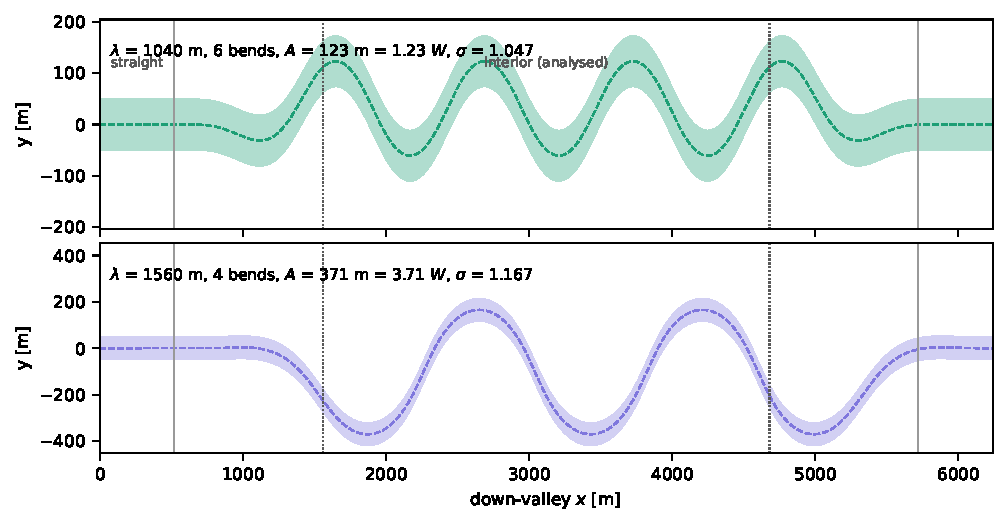
\includegraphics[width=\linewidth]{fig_plan.pdf}
  \caption{$xOy$ plan view of the two reaches. Both share the down-valley length
  $L$, the grid, the buffers, and the apex curvature $C_0=Ak^2$; only the bend
  \emph{density} differs. Dotted lines: buffer edges (non-erodible); solid grey lines:
  end of the straight lead-in. The lateral axis is exaggerated.}
  \label{fig:plan}
\end{figure}

\begin{figure}[t]
  \centering
  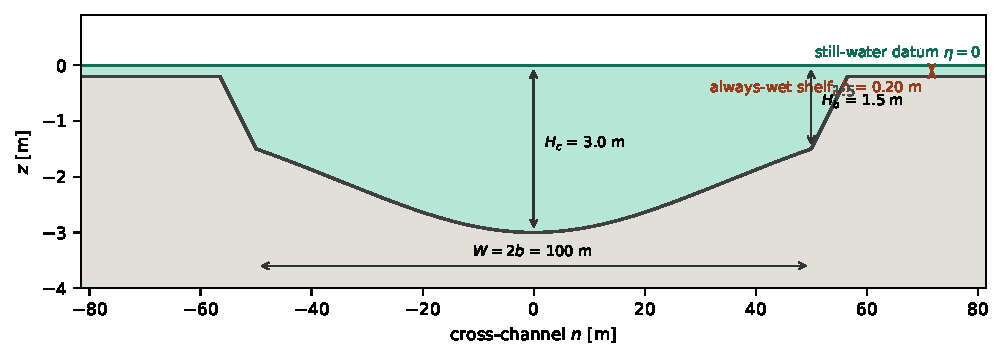
\includegraphics[width=\linewidth]{fig_section.pdf}
  \caption{$yOz$ cross-section \eqref{eq:section}, identical at every $s$. The
  constant-$\dn q$ bed occupies $|n|\le b$; beyond it the bank rises at $1{:}m$ to the
  floodplain. The gap between the still-water datum and the bank top is the freeboard
  analysed in \S\ref{sec:freeboard}.}
  \label{fig:section}
\end{figure}

% =====================================================================
\section{Boundary conditions}
\label{sec:bc}

\subsection{Inflow and outflow}
FUNWAVE's tide module relaxes \emph{all three} of $\eta$, $u$, $v$ toward prescribed
constants inside a sponge $I_w=30$ cells wide at each of the west and east boundaries
(\code{src/mod\_tide.F:323-330}):
\begin{equation}
  \phi \;\leftarrow\; \phi_{\rm BC} + \left(\phi-\phi_{\rm BC}\right)\Sigma(i),
  \qquad
  \Sigma=\left[\max\!\left(A_{sp}^{\,r},1\right)\right]^{-1},\quad
  r=R_{sp}^{\,50(i-1)/(I_w-1)},
  \label{eq:tidebc}
\end{equation}
with $R_{sp}=0.85$, $A_{sp}=10$. The imposed state is the uniform normal flow
\begin{equation}
  \eta_{\rm BC}=\pm\tfrac12 S L_{\rm ch},\qquad
  u_{\rm BC}=U \ \text{(west)},\qquad v_{\rm BC}=0 ,
  \label{eq:bcvals}
\end{equation}
$L_{\rm ch}=\sigma L$ being the channel (not valley) length. \textbf{Every component must
be given at both ends}: \code{TideEast\_U} defaults to zero (\code{src/mod\_tide.F:454}),
which walls the outflow.

\paragraph{Well-posedness caveat.} A subcritical open-channel reach admits \emph{one}
condition at the inlet (discharge) and \emph{one} at the outlet (stage). Equation
\eqref{eq:tidebc} imposes three at each. The extra conditions must therefore be made
mutually consistent, which is the purpose of the calibration in \S\ref{sec:head}. This is
the single largest practical difficulty in driving FUNWAVE as a river: no shipped example
uses steady discharge through-flow, so this operating point is untested territory for the
code.

\subsection{Banks: a free waterline, not a wall}
No boundary condition is applied at the banks. A cell is wet or dry by
\begin{equation}
  \mathrm{MASK}=
  \begin{cases} 1, & H>H_{\min}\\ 0, & H\le H_{\min}\end{cases}
  \qquad H_{\min}=0.01\ \mathrm{m},
  \label{eq:wetdry}
\end{equation}
and fluxes through a dry face vanish. The waterline is therefore free to move up and down
the bank, and \textbf{the channel width is not imposed} --- in contrast with the fixed-wall
condition $u_n(\pm b)=0$ of the linear $(s,n)$ model, which is only legitimate in the
limit of vanishing bank erodibility.

\paragraph{The alternative that was rejected.} FUNWAVE \emph{does} support true internal
vertical walls: \code{OBSTACLE\_FILE}$\to$\code{MASK\_STRUC}, with
\code{MASK\_STRUC = 0} a permanent dry point ($h=-\text{LARGE}$,
\code{src/init.F:1145-1151}). That reproduces $u_n(\pm b)=0$ exactly and needs no
elevation at all. It is not used here because \code{MASK\_STRUC} is never updated after
initialisation, so a vertical wall is necessarily a \emph{rigid} bank --- and bank erosion
is the point.

\subsection{Sediment}
\begin{equation}
  \text{advective scalar flux}=0 \quad\text{on all four open boundaries}
  \qquad(\code{mod\_sediment.F:1443-1503}),
\end{equation}
i.e.\ there is no equilibrium-inflow condition, and \code{PERIODIC} is south--north only
so no streamwise-periodic reach exists. The artefact this creates is quarantined by a
non-erodible buffer of \emph{fixed physical length} $\ell_b$ at each end:
\begin{equation}
  Z_s(x,y)=\begin{cases} 0, & x<\ell_b \ \text{or}\ x>L-\ell_b\\ \infty, & \text{otherwise,}\end{cases}
  \qquad Z_b \le Z_s .
  \label{eq:hardbottom}
\end{equation}
$\ell_b$ is a length and not a bend count because the artefact's scale is the sediment
adaptation length $L_a=UH/(\gamma w_s)\approx 20$ m plus the flow adjustment, neither of
which scales with $\lambda$.

\paragraph{$Z_s$ blocks erosion only.} It is applied as
\code{IF(Zb>Zs) Zb=Zs} with $Z_b>0$ meaning erosion, so deposition ($Z_b<0$) is
\emph{not} capped and the buffer does accrete. It is a quarantine, not a frozen bed, and
is excluded from analysis.

% =====================================================================
\section{Initial condition}

The analytic normal-flow state for the calibrated bed slope:
\begin{equation}
  \eta_0=-S\left(s-s_0\right),\qquad
  |\bm u_0|=\sqrt{\frac{g\,h_{\rm sec}\,S}{C_d}},\qquad
  \bm u_0=|\bm u_0|\,\hat{\bm t},
  \label{eq:ic}
\end{equation}
so that $H_0=\eta_0+h=h_{\rm sec}$ exactly: the initial depth is the design section
everywhere, and the surface parallels the bed. Starting from rest instead would cost a
full channel transit time, and because the two cases have different channel lengths that
would give them \emph{different} spin-up durations --- a confound in exactly the variable
under test. The run is therefore split into a rigid-bed spin-up
(\code{Bed\_Change = F}, one transit time, per-case) and a mobile-bed phase hot-started
from it through \code{INI\_UVZ} (identical duration for both cases).

% =====================================================================
\section{Sediment transport}
\label{sec:sed}

All stresses below are $\tau/\rho$; the density is divided out of both $\tau_b$ and
$\tau_{cr}$ in the source.

\begin{align}
  \text{bed shear (\code{:1254})}\qquad
    &\tau_b=\frac{\kappa^2|\bm u|^2}{\left[\ln(30H/k_s)-1\right]^2},
     \qquad \kappa^2=0.16,\quad k_s=2.5D_{50}, \label{eq:tau}\\
  \text{critical (\code{:936})}\qquad
    &\tau_{cr}=(s_g-1)\,g\,D_{50}\,\theta_{cr}, \label{eq:taucr}\\
  \text{grain parameter (\code{:935})}\qquad
    &D_*=D_{50}\left[\frac{(s_g-1)g}{\nu^2}\right]^{1/3}, \\
  \text{settling (Soulsby 1997)}\qquad
    &w_s=\frac{\nu}{D_{50}}\left[\sqrt{10.36^2+1.049D_*^3}-10.36\right]
     =0.0745\ \mathrm{m\,s^{-1}}.
\end{align}

\subsection{Erosion (pickup) --- van Rijn (1984), \code{:1287--1297}}
For $\tau_b>\tau_{cr}$ and $H>H_{\rm pick}$:
\begin{equation}
  c_b=0.015\left[\frac{\tau_b-\tau_{cr}}{\tau_{cr}}\right]^{3/2}D_*^{-0.3},
  \qquad
  c_a=\min\!\left(1,\frac{0.65}{c_b}\right)c_b\frac{D_{50}}{0.01H},
  \qquad
  \boxed{\;P=\max\left(0,\;c_a w_s\right).\;}
  \label{eq:pickup}
\end{equation}

\paragraph{$H_{\rm pick}$ is load-bearing.} The shipped example uses
$H_{\rm pick}=0.1$ m, which switches pickup off in shallow water --- that is, \emph{at the
bank toe}, which is the entire bank-retreat mechanism. It cannot be zero either: the log
law \eqref{eq:tau} is singular at $H=e\,k_s/30=1.13\times10^{-4}$ m. We use
$H_{\rm pick}=0.01$ m, $88\times$ above the singularity and $10\times$ below the example.

\subsection{Deposition --- Cao, \code{:1369--1372}}
\begin{equation}
  \gamma=\min\!\left[2,\;\frac{1-n_p}{\bar c}\right],
  \qquad
  \boxed{\;D=\gamma\,\bar c\,w_s\left(1-\gamma\bar c\right)^{2}.\;}
  \label{eq:depo}
\end{equation}

\paragraph{Erosion and deposition are both always on.} $P$ depends on $\tau_b$ and
\emph{not} on $\bar c$ (a pure source); $D$ is linear in $\bar c$ (a sink). They act
simultaneously at every wet point. The bed responds to the \emph{net} $D-P-\nabla\!\cdot\!\bm q_b$;
under capacity transport $D=P$ and the bed does not move. One cannot have erosion without
deposition: \eqref{eq:susp} would then have no sink and $\bar c$ would grow without bound.
Deposition is also what builds bars, so removing it would remove the phenomenon of interest.

\subsection{Suspended load}
\begin{equation}
  \dt\!\left(\bar c H\right) + \nabla\!\cdot\!\left(\bar c H\bm u\right)
  = \nabla\!\cdot\!\left(k H\nabla\bar c\right) + P - D .
  \label{eq:susp}
\end{equation}
Because $P$ is $\bar c$-independent and $D$ is linear in $\bar c$, \eqref{eq:susp} is a
relaxation equation with time and length scales
\begin{equation}
  T_c=\frac{H}{\gamma w_s}=20.1\ \mathrm{s},
  \qquad
  L_a=U\,T_c=20\ \mathrm{m}=0.20\,W .
  \label{eq:Tc}
\end{equation}

\subsection{Bedload --- Meyer-Peter \& M\"uller (1948), \code{:1319--1323}}
For $\tau_b>\tau_{cr}^{b}$:
\begin{equation}
  |\bm q_b|=\frac{8\left(\tau_b-\tau_{cr}^{b}\right)^{3/2}}{g\left(s_g-1\right)},
  \qquad
  \bm q_b=|\bm q_b|\,\big(\cos\alpha,\sin\alpha\big),
  \qquad \alpha=\operatorname{atan2}(v,u).
  \label{eq:bedload}
\end{equation}

% =====================================================================
\section{Bed and bank evolution}

\subsection{Exner}
\begin{equation}
  \boxed{\;\left(1-n_p\right)\dt z_b \;=\; D - P - \nabla\!\cdot\!\bm q_b\;}
  \label{eq:exner}
\end{equation}
implemented in cumulative form with $Z_b>0$ meaning erosion (\code{:1531--1546}):
\begin{equation}
  Z_b=-\frac{1}{1-n_p}\left[\int\!\left(\bar D-\bar P\right)\mathrm dt
       \;-\;\int\!\nabla\!\cdot\!\bm q_b\,\mathrm dt\right],
  \qquad Z_b\le Z_s,
\end{equation}
where $\bar P,\bar D$ are means over the window \code{Morph\_interval}. The bed seen by the
hydrodynamics is then
\begin{equation}
  h = h_{\rm ini} + Z_b\cdot \mathrm{MF},
  \qquad \mathrm{MF}\in\mathbb Z \ \text{(\code{Morph\_factor})}.
  \label{eq:mf}
\end{equation}

\subsection{Banks}
There is \textbf{no separate bank law}. A bank is an ordinary bed cell at the channel
margin and erodes through \eqref{eq:pickup}--\eqref{eq:exner} like any other. Bank
\emph{retreat} therefore has two ingredients:
\begin{enumerate}\itemsep2pt
  \item \textbf{toe erosion} --- \eqref{eq:exner} steepens the bank face;
  \item \textbf{geotechnical failure} --- wherever the local slope exceeds the angle of
        repose, material is moved down-slope (\code{:1554--1637}), every
        \code{Aval\_interval}:
        \begin{equation}
          \text{if }\ \max_{j\in\mathcal N(i)}\frac{z_{b,i}-z_{b,j}}{\Delta x}>\tan\phi
          \ \text{ and }\ Z_{b,i}<Z_{s,i}:\quad
          \delta=\tfrac12\left(z_{b,i}-z_{b,j}\right)-\tfrac12\tan\phi\,\Delta x,
        \end{equation}
        with $z_{b,i}\!\mathrel{-}=\delta$, $z_{b,j}\!\mathrel{+}=\delta$.
\end{enumerate}
This \emph{derives} bank retreat rather than prescribing it, but its rate is set by
$D_{50},\theta_{cr},\tan\phi$ --- \textbf{not} by an erodibility coefficient $E$. It is
therefore not comparable, without recalibration, with a kinematic law
$\dt\zeta_c=E\cdot\tfrac12[u_s'(+b)-u_s'(-b)]$.

% =====================================================================
\section{Head budget and its calibration}
\label{sec:head}

The straight-channel normal slope $S_0=C_dU^2/(gH_c)$ omits bend losses. Imposing it
together with the inlet velocity over-specifies the problem: the reach cannot pass the
design discharge on that head, draws down, loses conveyance, and diverges. The bed slope
and the boundary head are therefore scaled together by a calibrated factor,
\begin{equation}
  S = \mathcal H\,S_0,
  \qquad
  \mathcal H_{\rm new}=\mathcal H\left(\frac{U}{U_{\rm meas}}\right)^{2},
  \label{eq:hf}
\end{equation}
the update following from $U\propto\sqrt S$. Scaling \emph{both} keeps the state
self-consistent ($H=h_{\rm sec}$ at uniform flow). Measured: $U\propto\sqrt S$ holds to
$0.8\%$, and the reach delivers $\approx82\%$ of the straight-channel target, i.e.
$\mathcal H\approx1.5$ at $R/W=2$.

% =====================================================================
\section{Will the water leave the channel?}
\label{sec:freeboard}

No. The free surface is bounded by the imposed head drop plus the bend superelevation:
\begin{equation}
  \boxed{\;\eta_{\max}\;\simeq\;\tfrac12 S\,L_{\rm ch} \;+\; \frac{U^2W}{2gR}
  \;<\; f \quad\text{(bank top)}.\;}
  \label{eq:freeboard}
\end{equation}
For the present configuration:
\begin{center}
\begin{tabular}{lcccc}
\toprule
case & $\tfrac12 S L_{\rm ch}$ & superelevation $/2$ & $\eta_{\max}$ & margin to $f=1.5$ m \\
\midrule
$\lambda=1040$ m & $0.154$ m & $0.018$ m & $0.172$ m & $1.328$ m \ ($8.7\times$) \\
$\lambda=520$ m  & $0.129$ m & $0.018$ m & $0.147$ m & $1.353$ m \ ($10.2\times$) \\
\bottomrule
\end{tabular}
\end{center}
The flow is confined to the channel and erosion is restricted to the bed and the banks, as
intended. Note that the observed failure mode in the unstable configurations is the
\emph{opposite} of overflow: the reach \emph{drains} ($\eta\to-73$ m in one case), which
FUNWAVE does not flag because its blow-up threshold is $100\times$ the maximum depth. Run
health must therefore be judged on the fields --- fraction of the channel still wet, and
$|\eta|$ inside the channel --- never on the string \code{Normal Termination}.

% =====================================================================
\section{Timescales}
\label{sec:timescales}

\begin{equation}
  T_{\rm flow}=\frac{\mathrm{CFL}\,\Delta x}{U+\sqrt{gH}},\qquad
  T_c=\frac{H}{\gamma w_s},\qquad
  T_{\rm bed}=\frac{(1-n_p)H\,\mathcal L}{q_b},\qquad
  T_{\rm bank}=\frac{b}{\varepsilon U}.
\end{equation}
At $U=0.85\ \mathrm{m\,s^{-1}}$, $D_{50}=0.5$ mm:
\begin{center}
\begin{tabular}{lcccc}
\toprule
 & $T_{\rm flow}$ & $T_c$ & $T_{\rm bed}$ (one bar) & $T_{\rm bank}$ \\
\midrule
value & $0.20$ s & $20.1$ s & $1.68\times10^{7}$ s $=194$ d & $\sim5\times10^{9}$ s \\
\bottomrule
\end{tabular}
\end{center}
Two consequences. (i) \code{Morph\_interval} must exceed $T_c$ by a good margin or the
Exner forcing is an unequilibrated suspension transient; we use $200$ s $\approx10\,T_c$.
(ii) $T_{\rm bed}/T_{\rm flow}\sim10^{8}$, bridged by $\mathrm{MF}=1000$ in \eqref{eq:mf};
$T_{\rm bank}$ is a further factor beyond and is \emph{not} reachable, so this model gives
bar and bend morphodynamics, not century-scale planform migration.


% =====================================================================
\section{Complete list of approximations}
\label{sec:approx}

This model is \textbf{not} a first-principles simulation. Every approximation it makes is
listed here; results can only be read through this list.

\subsection{Physical}
\begin{enumerate}\itemsep1pt
  \item \textbf{Hydrostatic pressure}, $p=\rho g(\eta-z)$: the long-wave limit $L\gg H$.
        Vertical accelerations are neglected.
  \item \textbf{Depth-averaged}: no vertical coordinate. Secondary (helical) circulation
        cannot exist, so \eqref{eq:secondary} is identically absent and $A_s=0$.
  \item \textbf{Non-dispersive}: \code{DISPERSION = F} drops all Boussinesq terms
        ($\Gamma_1=\Gamma_2=0$). Valid because $kH\ll1$ for a river.
  \item \textbf{Non-rotating}, $f=0$. Any ``Rossby wave'' here is a shear-$\beta$ vortical
        wave, never a planetary one.
  \item \textbf{Uniform, non-cohesive grain size} $D_{50}$: no grading, no armouring, no
        cohesion, no bedforms (ripples/dunes are inside $k_s=2.5D_{50}$, not resolved).
  \item \textbf{Empirical transport closures}: log-law drag \eqref{eq:tau}, van~Rijn
        pickup \eqref{eq:pickup}, Cao deposition \eqref{eq:depo}, Meyer-Peter--M\"uller
        bedload \eqref{eq:bedload}, Soulsby settling. Each carries its own calibration
        range; none is derived.
  \item \textbf{Bedload direction $=$ depth-averaged flow direction}. No gravitational
        deflection down the transverse slope \eqref{eq:slopedefl}.
  \item \textbf{Smagorinsky eddy viscosity} \eqref{eq:smag} as the sole lateral closure.
  \item \textbf{Avalanching is instantaneous} relaxation to $\tan\phi$ once per
        \code{Aval\_interval}; no soil mechanics, no pore pressure, no cohesion.
  \item \textbf{Rigid, impermeable floodplain}: no infiltration, no overbank sediment.
\end{enumerate}

\subsection{Timescale separation --- the model is \emph{not} fully coupled}
\label{sec:approx-time}
This is the largest approximation and it is deliberate.
\begin{enumerate}\setcounter{enumi}{10}\itemsep1pt
  \item \textbf{Morphological acceleration}, $\mathrm{MF}=1000$ in \eqref{eq:mf}. The bed
        is advanced a thousand times faster than the flow that drives it. Formally this
        assumes the flow is slaved to the bed --- valid when the bed moves negligibly over
        a hydrodynamic adjustment time, which \S\ref{sec:timescales} supports
        ($T_{\rm bed}/T_{\rm flow}\sim10^8$) but which \textbf{must be verified by an
        MF-convergence sweep}, not assumed.
  \item \textbf{Time-averaged Exner forcing}: $P$ and $D$ are averaged over
        \code{Morph\_interval} $=200\ \mathrm s\approx10\,T_c$ before they move the bed
        \eqref{eq:exner}. This is exactly the ``average over the fast timescale, then
        erode'' step; it filters suspension transients out of the bed forcing.
  \item \textbf{$\dt h$ dropped from the hydrodynamic mass equation} \eqref{eq:mass}: the
        flow does not see the bed moving \emph{within} a hydrodynamic step, only between
        bed updates.
  \item \textbf{Rigid-bed spin-up}: phase~1 runs with \code{Bed\_Change = F}, i.e.\ the
        bed and banks are literally rigid on the fast timescale, and the mobile-bed phase
        is hot-started from the converged flow.
\end{enumerate}
Items 11--14 together \emph{are} a fast/slow decomposition. A stronger, fully decoupled
alternative is discussed in \S\ref{sec:decouple}.

\subsection{Numerical}
\begin{enumerate}\setcounter{enumi}{14}\itemsep1pt
  \item \textbf{Finite resolution} $\Delta x=\Delta y=2.5$ m: 40 cells across the channel,
        6 across the bank face. The bank is a staircase at this resolution.
  \item \textbf{MUSCL--TVD reconstruction with an HLL Riemann solver}, third order in
        space; the limiter is diffusive at extrema.
  \item \textbf{Wetting--drying threshold} $H_{\min}=0.01$ m and the friction floor
        $H_{\rm frc}$; a cell below threshold is removed from the solution and its water
        is booked into a mass-adjustment term.
  \item \textbf{Pickup floor} $H_{\rm pick}=0.01$ m: no entrainment in water shallower
        than this, a numerical necessity because \eqref{eq:tau} is singular at
        $H=e\,k_s/30$.
  \item \textbf{Sediment is closed at the open boundaries}, worked around by the
        non-erodible buffer \eqref{eq:hardbottom}; the buffer is excluded from analysis.
  \item \textbf{The boundary condition is over-specified} (\S\ref{sec:bc}) and made
        consistent only by the head calibration \eqref{eq:hf}, which is itself an
        iterative, empirical procedure.
  \item \textbf{Geometry is modified inside the buffer} by the amplitude taper
        \eqref{eq:taper}: the first and last $\ell_b$ of the reach are not the meander
        being studied.
\end{enumerate}

% =====================================================================
\section{A fully decoupled alternative}
\label{sec:decouple}

Items 11--14 accelerate the bed while leaving the two systems dynamically coupled at every
step. In the strongly separated regime of \S\ref{sec:timescales} a cleaner scheme is
available, in which the fast problem is solved to \emph{steady state} before the slow one
is touched:
\begin{align}
  &\text{(i) freeze the bed; integrate \eqref{eq:mass}--\eqref{eq:momy}
        to a steady state } (\bm u^\ast,\eta^\ast);\notag\\
  &\text{(ii) time-average over the last several }T_c
        \Rightarrow \langle\bm u\rangle,\langle\eta\rangle;\notag\\
  &\text{(iii) evaluate } P,D,\bm q_b \text{ from } \langle\bm u\rangle
        \text{ only};\notag\\
  &\text{(iv) advance \eqref{eq:exner} by one explicit morphological step }
        \Delta t_m;\notag\\
  &\text{(v) rebuild } h \text{ and return to (i).}\notag
\end{align}
This is more rigorous than \eqref{eq:mf} in three ways: the sediment is computed from a
genuinely steady flow rather than from a partially-adjusted one; $\Delta t_m$ is explicit
and its convergence directly testable; and no feedback instability can arise from the bed
outrunning the flow. Its cost is one flow re-convergence per morphological step, which
from a hot start is short.

It also unlocks a diagnostic that the accelerated scheme cannot provide --- see
\S\ref{sec:dispersion}.

% =====================================================================
\section{Can a dispersion relation be extracted?}
\label{sec:dispersion}

\paragraph{Not from a nonlinear initial-value run.} Eigenmodes, $\sigma(k)$ and $c(k)$ are
properties of a \emph{linear operator}. Equations \eqref{eq:mass}--\eqref{eq:momy} are
integrated nonlinearly, superposition does not hold, and a single run therefore contains no
dispersion relation. The linear $(s,n)$ package obtains one because it linearises about a
frozen base state; that route is closed here by construction.

\paragraph{The hydrodynamic question is already settled, and negatively.} Whether the
meander is a gravity wave or a vortical (shear-$\beta$) wave was tested in the linear
package and the vortical claim was \emph{retracted}: every growing run had
$T_{\rm shear}\le0$, i.e.\ the growing disturbance \emph{loses} energy to the mean flow.
Moreover the Froude test is analytically null --- writing $P\equiv g\eta$, the momentum
equations contain no $F$ and $F$ survives only as $F^2$ multiplying the continuity time
derivative, so $F$-insensitivity confirms the rigid-lid reduction rather than
discriminating wave families. A nonlinear solver cannot improve on either result.

\paragraph{What \emph{can} be measured, and is worth measuring.} The productive question
is not gravity-versus-Rossby but \emph{free morphodynamic (alternate-bar) mode versus
forced boundary mode}, and for that a dispersion relation can be built numerically from
the decoupled scheme of \S\ref{sec:decouple} by finite-differencing the nonlinear operator:
\begin{enumerate}\itemsep1pt
  \item start from a straight channel at equilibrium;
  \item perturb the bed by a small sinusoid,
        $z_b\to z_b+\epsilon\sin(kx)\,\Phi(n)$, with $\epsilon\ll H$;
  \item run step (i)--(iii) of \S\ref{sec:decouple} to get $\nabla\!\cdot\!\bm q_b$ from
        the re-converged steady flow;
  \item project the response onto mode $k$ and form
        \begin{equation}
          \sigma(k) \;=\; -\frac{1}{(1-n_p)\,\epsilon}
          \left\langle \nabla\!\cdot\!\bm q_b - D + P,\; \sin(kx)\Phi(n)\right\rangle ,
        \end{equation}
        the growth rate of the morphodynamic mode; the quadrature phase gives the
        migration speed $c(k)$;
  \item repeat over $k$ and over $\epsilon$ to confirm linearity.
\end{enumerate}
This is a genuine, numerically-obtained dispersion relation for the \emph{bed}, which is
the quantity that bar theory predicts and that selects $\lambda$. It requires the closures
of \S\ref{sec:notcontain}: with $A_s=0$ and no slope deflection there is no free bar mode
to find, so \eqref{eq:slopedefl}--\eqref{eq:secondary} are a prerequisite, not an optional
refinement.

% =====================================================================
\section{What the model does not contain}
\label{sec:notcontain}

Two closures are absent from \eqref{eq:bedload}, and together they are what builds a point
bar:
\begin{align}
  \text{transverse bed-slope deflection}\qquad
    &q_{b,n}=|\bm q_b|\left[\sin\alpha-\frac{1}{f(\theta)}\dn z_b\right], \label{eq:slopedefl}\\
  \text{secondary (helical) flow}\qquad
    &\tan\delta=A_s\frac{H}{R_s} . \label{eq:secondary}
\end{align}
Stock FUNWAVE directs bedload along $\operatorname{atan2}(v,u)$ and nothing else, so
$A_s=0$ and there is no gravitational return of grains down the transverse slope. In the
classification of Ikeda, Parker \& Sawai (1981) this is their $A=0$ case, which they
identify with \emph{incised} rather than alluvial meanders; their alluvial value is
$A\approx2.89$.

\begin{quote}\itshape
Standing prediction, registered before the runs: outer-bank scour \emph{without} an inner
point bar. \code{postprocessing/01\_validate.py} reports the measured inner/outer bed
change split against it.
\end{quote}

Also absent: any vertical structure (the model is depth-averaged, hence
\eqref{eq:secondary} cannot arise on its own); rotation ($f=0$, so ``Rossby wave''
here can only mean a shear-$\beta$ vortical wave, never a planetary one); along-channel
depth variation in the initial bed ($h$ depends on $n$ only, plus the uniform tilt --- any
$h(x)$ structure must \emph{emerge} from \eqref{eq:exner}); and width variation as an
independent parameter.

\end{document}
